% !TeX spellcheck = da_DK
% Setup document class.
%  This will always be the beamer class, but depending on the use of notes,
%  it can be annotated with the option [notes] or  [notes=only], depending
%  on whether notes should be included, or should be the only thing in
%  the document.

\documentclass[xcolor=table]{beamer}

%%%% USE WHEN PRINING HANDOUTS %%%%%

%\documentclass[xcolor=table, handout]{beamer}
%\usepackage{pgfpages}
%\pgfpagesuselayout{2 on 1}[a4paper,border shrink=5mm]

%%%%%%%


% Setup theme.
%\usetheme[
%%% options passed to the outer theme
%    progressstyle=fixedCircCnt,   %either fixedCircCnt, movCircCnt, or corner
%    rotationcw,          % change the rotation direction from counter-clockwise to clockwise
%    shownavsym          % show the navigation symbols
]{AAUsimple}

\usetheme[
%%% options passed to the outer theme
%    hidetitle,           % hide the (short) title in the sidebar
%    hideauthor,          % hide the (short) author in the sidebar
%    hideinstitute,       % hide the (short) institute in the bottom of the sidebar
%    shownavsym,          % show the navigation symbols
%    width=2cm,           % width of the sidebar (default is 2 cm)
    hideothersubsections,% hide all subsections but the subsections in the current section
%    hideallsubsections,  % hide all subsections
    left               % right of left position of sidebar (default is right)
%%% options passed to the color theme
%    lightheaderbg,       % use a light header background
  ]{AAUsidebar}

\setbeamercolor{alerted text}{fg=blue,bg=}


% Import preamble
%%% Initial things %%%
% Increase number of dimen registers
\usepackage{etex}
% Fix various issues with LaTeX2e
\usepackage{fixltx2e}
% Font package
\usepackage{fourier}


%%% Translations and character encodings %%%
% Enable use of several characters, including æ, ø and å
\usepackage[utf8]{inputenc}
% Danish language
\usepackage[danish]{babel}
% Use PostScript fonts instead of bitmap ones. Also does other stuff.
\usepackage[T1]{fontenc}
% Various LaTeX symbols
\usepackage{latexsym}
% Wider selection of colours
\usepackage{xcolor}
% Improved element justification
\usepackage{ragged2e}
% Font improvements
\usepackage{fix-cm}
% Enables various forms of lines, like double-underlining (\uuline{})
\usepackage{ulem}
% Sets the tolerance for distance between words, determining when to hyphenate.
\pretolerance=2500

\usepackage{rotating}

%%% Figures and tables (Floats) %%%
% Enable multi-rows and -columns
\usepackage{multirow}
\usepackage{multicol}
% Double, horizontal lines
\usepackage{hhline}
% Enables coloured tables
\usepackage{colortbl}
% Prettier tables
\usepackage{booktabs}


%%% Mathematic formulas %%%
% AMS math
\usepackage{amsmath}
\usepackage{amssymb}
% Extra fonts (for math, I think)
\usepackage{stmaryrd}
% Access text symbols
\usepackage{textcomp}
% Extend AMS
\usepackage{mathtools}
\usepackage{cancel}


%%% Graphics %%%
% Various image-commands
\usepackage{eso-pic}
% Use JPEG and PNG images
\usepackage{graphicx}

%%% Code listing %%%
\usepackage{color}
\definecolor{bluekeywords}{rgb}{0.13,0.13,1}
\definecolor{greencomments}{rgb}{0,0.5,0}
\definecolor{redstrings}{rgb}{0.9,0,0}

\usepackage{courier}

\usepackage{listings}

\lstset{language=[Sharp]C,
  captionpos=b,
  columns=fixed,
  numbers=left,
  numberstyle=\tiny,
  showspaces=false,
  showtabs=false,
  tabsize=3,
  breaklines=true,
  inputencoding=utf8,
  showstringspaces=false,
  breakatwhitespace=true,
  escapeinside={(*@}{@*)},
  commentstyle=\color{greencomments},
  keywordstyle=\color{bluekeywords},
  stringstyle=\color{redstrings},
  basicstyle=\ttfamily\small,
}

\lstdefinestyle{make}{tabsize=2}


%%% References, bibtex and URLs %%%
% Post URLs. Allows breaking at hyphens to help avoid long links.
\usepackage{url}
% Better cross references
\usepackage[danish]{varioref}
% Define a new 'leo' style for URL package, that will use a smaller font
\makeatletter
\def\url@leostyle{%
  \@ifundefined{selectfont}{\def\UrlFont{\sf}}{\def\UrlFont{\small\ttfamily}}
}
\makeatother
% And of course, use this new style
\urlstyle{leo}

\hypersetup{pdfstartview={Fit}}
%%%%%%%%%%%%%%%%%%%%%%%%%%%%%%%%%%%%%%%%%%%%%%%%
%Flowchart
\usepackage{tikz}
\usetikzlibrary{shapes.geometric, arrows, positioning}
%%%%%%%%%%%%%%%%%%%%%%%%%%%%%%%%%%%%%%%%%%%%%%%%



\usepackage{color}
\definecolor{bluekeywords}{rgb}{0.13,0.13,1}
\definecolor{greencomments}{rgb}{0,0.5,0}
\definecolor{redstrings}{rgb}{0.9,0,0}
\usepackage{courier}
\usepackage{listings}

\lstset{ 
    literate={ø}{{\o}}1
         {æ}{{\ae}}1
         {å}{{\aa}}1
         {Ø}{{\O}}1
         {Æ}{{\AE}}1
         {Å}{{\AA}}1
         {§}{{\S}}1
}

%%% Colour definitions %%%
% Defines: gray
\definecolor{gray}{gray}{0.80}
% Defines: numbercolor
\definecolor{numbercolor}{gray}{0.7}
% Defines: shadecolor
\definecolor{shadecolor}{RGB}{33,26,82}
% Defines: aaublue

\definecolor{aaublue}{RGB}{33,26,82}


\colorlet{punct}{red!60!black}
\definecolor{background}{HTML}{EEEEEE}
\definecolor{delim}{RGB}{20,105,176}
\colorlet{numb}{magenta!60!black}

\newcommand*\rot{\rotatebox{90}}


% Additional settings for boxes
\setbeamercolor{headerCol}{fg=black,bg=lightgray}
\setbeamercolor{bodyCol}{fg=white,bg=gray}
\setbeamercovered{transparent=20}

% Define document stuff
\title[GAMBL]{GAMBL}
\subtitle[Eksamen]{Eksamen}
\author[SW413F15]{Gruppe SW413F15}
\date{26. Juni 2015}

\institute[
%  {\includegraphics[scale=0.2]{aau_segl}}\\ %insert a company, department or university logo
Software (SW4)\\
Aalborg Universitet\\
Danmark
] % optional - is placed in the bottom of the sidebar on every slide
{% is placed on the title page
  Software (SW4)\\
  Aalborg Universitet\\
  Danmark
  
  %there must be an empty line above this line - otherwise some unwanted space is added between the university and the country (I do not know why;( )
}

% Specify a logo on the titlepage (you can specify additional logos an include them in 
% institute command below
\pgfdeclareimage[height=1.5cm]{titlepagelogo}{AAUgraphics/aau_logo_new} % placed on the title page
%\pgfdeclareimage[height=1.5cm]{titlepagelogo2}{graphics/aau_logo_new} % placed on the title page
\titlegraphic{% is placed on the bottom of the title page
  \pgfuseimage{titlepagelogo}
  %  \hspace{1cm}\pgfuseimage{titlepagelogo2}
}


\begin{document}

{\aauwavesbg
  \begin{frame}[plain,noframenumbering]
    \titlepage
  \end{frame}}

% ==================== SUBJECTS ======================
\input{slides/corlin.tex}
\section{Scanner and Parser Generators}
\begin{frame}{Scanner and Parser Generators}
  \begin{itemize}
    \item Parser overview
    \item Parser generators
    \item Lexer
    \item CFG
  \end{itemize}
\end{frame}

\begin{frame}{Parser overview}
  Automate the generation of lexer and parser.
\begin{figure}[ht]
\centering
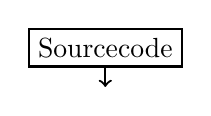
\begin{tikzpicture}
  \draw [thick, ->] (0,0.3) -- (0,0);
  \node [rectangle, draw, thick,fill=white!20] at (0,0.5) {Sourcecode};
\end{tikzpicture}

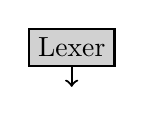
\begin{tikzpicture}
  \draw [thick, ->] (0,0.3) -- (0,0);
  \node [rectangle, draw, thick,fill=gray!90] at (0,0.5) {Lexer};
\end{tikzpicture}


\begin{tikzpicture}
  \draw [thick, ->] (0,0.3) -- (0,0);
  \node [rectangle, draw, thick,fill=white!20] at (0,0.5) {Token stream};
\end{tikzpicture}

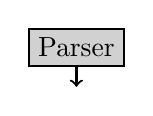
\begin{tikzpicture}
  \draw [thick, ->] (0,0.3) -- (0,0);
  \node [rectangle, draw, thick,fill=gray!90] at (0,0.5) {Parser};
\end{tikzpicture}

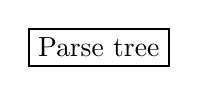
\begin{tikzpicture}
  \node [rectangle, draw, thick,fill=white!20] at (0,0.5) {Parse tree};
\end{tikzpicture}
\end{figure}
\end{frame}

\subsection{Parser Generators}
\begin{frame}{Parser Generators}
  \framesubtitle{Different parser generators}
  \begin{itemize}
    \item SableCC
    \item JavaCup
    \item ANTLR
    \item Coco/R
    \item Yacc
    \item And many mores.
  \end{itemize}
\end{frame}

\begin{frame}{SableCC}
  \begin{itemize}
    \item OO java compiler compiler
    \begin{itemize}
      \item also exsist as c++ and c\#
    \end{itemize}
    \item Input
    \begin{itemize}
      \item Token rules
      \item Grammar productions
    \end{itemize}
    \item Output
    \begin{itemize}
      \item Lexer
      \item Parser
      \item AST classes
      \item AST walkers
    \end{itemize}
  \end{itemize}
\end{frame}

\begin{frame}{JavaCup}
  \begin{itemize}
    \item Java LALR(1) parser generator
    \begin{itemize}
      \item Does not include lexer generator
    \end{itemize}
    \item Input
    \begin{itemize}
      \item Grammar productions
    \end{itemize}
    \item Output
    \begin{itemize}
      \item Parser
      \item optional action code
    \end{itemize}
  \end{itemize}
\end{frame}

\begin{frame}{ANTLR}
 \begin{itemize}
    \item Java LL(*) parser generator
    \begin{itemize}
      \item Can be used with ANTLRWorks IDE
    \end{itemize}
    \item Input
    \begin{itemize}
      \item Token rules
      \item Grammar productions
    \end{itemize}
    \item Output
    \begin{itemize}
      \item Lexer
      \item Parser
      \item Error Reporting
    \end{itemize}
  \end{itemize}
\end{frame}

\subsection{Tokens and Lexer}
\begin{frame}{Tokens}
  \begin{itemize}
    \item TOKENS!
  \end{itemize}
\end{frame}

\begin{frame}{Lexer}

\end{frame}


\subsection{CFG}
\begin{frame}{GAMBL's CFG}

\end{frame}

\begin{frame}{Alternative CFG}

\end{frame}

\section{Semantics}

\begin{frame}{Semantics}
\framesubtitle{Type Checking}

\begin{itemize}
  \item Lack of Type checking in semantics
  \item Matrices and Vectors
\end{itemize}

\begin{equation}
\small
\frac { { e }_{ v },st\vdash { a }_{ 1 }{ \rightarrow  }_{ A }{ v }_{ 1 }\quad { e }_{ v },st\vdash { a }_{ 2 }{ \rightarrow  }_{ A }{ v }_{ 2 } }{ { e }_{ v },st\vdash { a }_{ 1 }+{ a }_{ 2 }{ \rightarrow  }_{ A }{ v } } ,\begin{matrix} v={ v }_{ 1 }+{ v }_{ 2 }, \\ Typeof({ a }_{ 1 }) = Typeof({ a }_{ 2 }) \end{matrix}
\end{equation}
\end{frame}

\begin{frame}{Booleans}
\framesubtitle{Booleans allowed in boolean expression}
\begin{equation}
	\frac { { e }_{ v },st\vdash { a }_{ 1 }{ \rightarrow  }_{ A }{ v }_{ 1 }\quad { e }_{ v },st\vdash { a }_{ 2 }{ \rightarrow  }_{ A }{ v }_{ 2 } }{ { e }_{ v },st\vdash { a }_{ 1 }=={ a }_{ 2 }{ \rightarrow  }true } ,{ v }_{ 1 }={ v }_{ 2 }
\end{equation}

\begin{equation}
	\frac { { e }_{ v },st\vdash { b }_{ 1 }{ \rightarrow  }_{ B }{ B }_{  }\quad { e }_{ v },st\vdash { b }_{ 2 }{ \rightarrow  }_{ B }{ B }_{  } }{ { e }_{ v },st\vdash { b }_{ 1 }=={ b }_{ 2 }{ \rightarrow  }true } 
\end{equation}

\begin{equation}
	\frac { { e }_{ v },st\vdash { b }_{ 1 }{ \rightarrow  }_{ B }{ B }_{ 1 }\quad { e }_{ v },st\vdash { b }_{ 2 }{ \rightarrow  }_{ B }{ B }_{ 2 } }{ { e }_{ v },st\vdash { b }_{ 1 }=={ b }_{ 2 }{ \rightarrow  }false } , { B }_{ 1 } \neq { B }_{ 2 } 
\end{equation}
\end{frame}

\section{Compiler}

    \subsection{Compiler vs. Intrepreter}
    \begin{frame}[t]{Compiler}\framesubtitle{Compiler vs. Intrepreter}
        \begin{itemize}
            \item Performance
            \item Development Cycle
            \item Debugging
            \item Specific Constraints
        \end{itemize}
    \end{frame}

    \subsection{Compiler Overview}
    \begin{frame}[t]{Compiler}\framesubtitle{Compiler Overview}
        \begin{columns}[t]
            \begin{column}{.48\textwidth}
                \begin{itemize}
                    \item ANTLRv4
                    \item Visitor Pattern
                    \item JAVA
                \end{itemize}
        \begin{figure}[ht]
        \centering
        \resizebox{.9\textwidth}{!}{
        \begin{tikzpicture}
            \matrix (m) [ampersand replacement=\&,matrix of nodes]
            {
             GAMBL  \& $\to$ \&  OpenCL C  \\
                \&  Java    \& OpenCL C \& $\to$ \& \hspace{1 em} M \hspace{2 em}  \\
                \&       \&   \& C  \&         \\
                \&       \&               \\
              };
            \draw (m-1-1.south west) |- (m-1-3.north east) |- (m-2-2.north east) |- (m-2-2.south west) |- (m-1-1.south west);
            \draw (m-2-2.south east) |- (m-2-5.north east) --(m-2-5.south east) -- (m-2-5.south west) |- (m-3-4.south west) |- (m-2-2.south east);
        \end{tikzpicture}
        }
        \end{figure}

            \end{column}
            \begin{column}{.48\textwidth}
                \vspace{-30pt}
                \begin{figure}
                    \centering
                    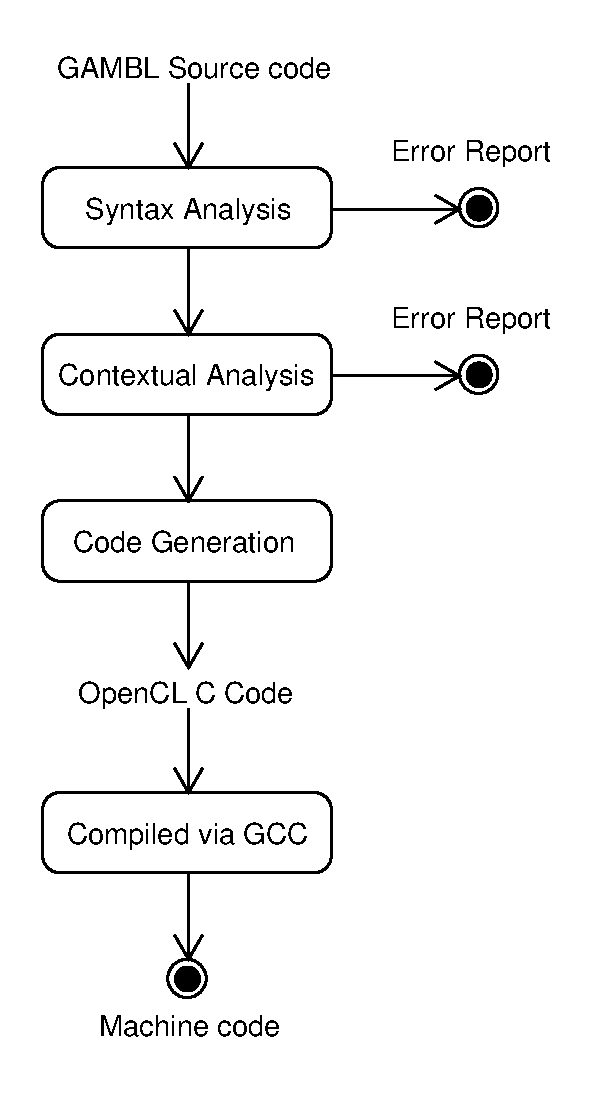
\includegraphics[width=0.8\textwidth]{images/CompilerDiagram.pdf}
                \end{figure}
            \end{column}
        \end{columns}
    \end{frame}
\section{temp}
\subsection{Visitor Pattern}
\begin{frame}{Traversing the Tree}
\framesubtitle{Visitor Pattern}
	\begin{itemize}
        \item ANTLR visitor pattern
        \item Our own Visitor Pattern
    \end{itemize}
    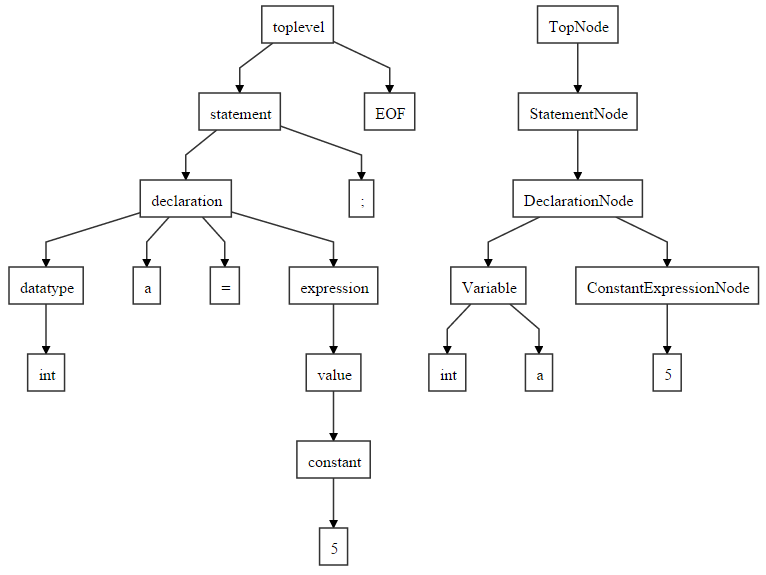
\includegraphics[width=1\textwidth,height=0.7\textheight,keepaspectratio, , clip]{images/P4/AST.PNG}

\end{frame}

\begin{frame}{Contextual Analysis}
\framesubtitle{Module call}

    \begin{lstlisting}
ContextualAnalyser contextualAnalyser = new ContextualAnalyser(inputFile, errors);
abstractSyntaxTree = contextualAnalyser.GenerateDecoratedASTFromParseTree(abstractSyntaxTree);
    \end{lstlisting}


\end{frame}

\begin{frame}{Contextual Analysis}
\framesubtitle{Module call}

\begin{lstlisting}
public BaseASTNode GenerateDecoratedASTFromParseTree(BaseASTNode abstractSyntaxTree){

  //Add potential imported function declarations
  handleImports(abstractSyntaxTree);

  //Scope check
  SymbolTable symbolTable = new SymbolTable();
  scopeCheck(abstractSyntaxTree, symbolTable);
  //Type check
  typeCheck(abstractSyntaxTree, symbolTable);

  //Check for unused variables
  errors.addAll(symbolTable.getUnusedVariables());

  //Error Handling
  ErrorReporter errorReporter = new ErrorReporter();
  errorReporter.HandleErrors(errors, ErrorType.ALL);

  return abstractSyntaxTree;
}
\end{lstlisting}

\end{frame}
\section{Demonstration} % (fold)
\label{sec:demonstration}
\begin{frame}{Demonstration}
    \begin{itemize}
        \item GAMBL toolchain
        \item Compilation of GAMBL sourcecode
        \begin{itemize}
            \item Compile-time errors
            \item Run-time errors
            \item Error free
        \end{itemize}
        \item Looking at output
        \begin{itemize}
            \item Target language
            \item Makefile
        \end{itemize}
    \end{itemize}
\end{frame}

% section demonstration (end)
\section{Project Review}

	\subsection{Discussion}
	\begin{frame}[t]{Project Review}\framesubtitle{Parallel Computing Platform}
		\begin{itemize}
			\item OpenCL
			%Different supported versions for each manufacturer
			\item CUDA
			%
			\item Operating Systems
			%WindowsNoWork, manual library and platform linking
		\end{itemize}
	\end{frame}

	\begin{frame}[t]{Project Review}\framesubtitle{Seamless GPU Usage}
		\begin{itemize}
			\item User Control
			%Brugeren har 0 kontrol over fordeling
			\item Predefined Operations
			%Kun enkelte predefinerede operationer udregnes på GPU, og for disse er der intet alternatitv der tillader brug af CPU
			\item Effeciency
			%I forhold til de steder hvor GPU udnyttes kontra andre steder den måske kunne udnyttes
		\end{itemize}
	\end{frame}

	\subsection{Conclusion}
	\begin{frame}[t]{Project Review}\framesubtitle{Conclusion}
		\begin{itemize}
		%Eventuelt starte med problemformulering/sprog kriterier?
			\item Seamless GPU utilisation
			 %+Read and writability
			\item Runtime Efficiency
			\item Error Reporting
			\item Cross Platform Solution vs. Single Platform Development 
			%Laves eventuelt om til eget slide
			\item Development Process
			%IterativUdvikling
		\end{itemize}
	\end{frame}

	\subsection{Future Works}
	\begin{frame}[t]{Project Review}\framesubtitle{Future Works}
		\begin{itemize}
			\item Linear Algebra
			%Mere end blot simple matrix operationer kunne være til gavn for programmøren 
			\item Code Analysis And User Control
			%Bedre fordeling af udregninger på platforme, både nativt og explicit har mulighed for at øge runtime efficiency i stor grad, muligheden for explicit gpu brug tillader desuden brugen flere steder end nativt, blot tradeoff er ansvar på bruger
			\item Kernel Improvements
			%Bedre brug af memory, platform targeting virker yderligere her dat Nvidia har anderledes architectur(Warps i thread hierarchy(thread>warp>ThreadBlock>Grid/Thread>WorkGroup>NDRange))
			%Possible improvements instead of Templates?(making functions available)
			\item Platform Targeting
			\item Research Fields
			\begin{itemize}
				\item Data Structures
				\item Functions
				\item Operations
				\item Algorithms
			\end{itemize}
		\end{itemize}
	\end{frame}


% ====================================================

% Final slide
{\aauwavesbg
  \begin{frame}[plain,noframenumbering]
    \finalpage{\texttt{throw new PresentationIsOverException();}}
  \end{frame}}

\end{document}
